% Festlegen des Dokumententyps
\documentclass[a4paper,twoside]{article}

% Papierformat
\usepackage{a4}

% Deutsche Sprache (Silbentrennung, usw.)
\usepackage[ngerman]{babel}

% Schrifteneinstellungen
\usepackage{lmodern}
\usepackage[T1]{fontenc}
\usepackage{textcomp}

% Kodierung
\usepackage{ucs}
\usepackage[utf8]{inputenc}

% bessere Matheunterstützung
\usepackage{amsfonts}
\usepackage{amstext}
\usepackage{amsmath}

% Einheiten in Formalen
\usepackage{siunitx}

% fuer Zitate
\usepackage{cite}

% Grafiken einbinden
\usepackage{graphicx}


% Verweise in PDF-Dateien
\usepackage
[colorlinks,
pdfstartview = 1,
bookmarksopen = true,
bookmarksnumbered = true,
linkcolor = black,
plainpages = true,
hypertexnames = false,
citecolor = black]{hyperref} 

\newcommand{\e}{{\rm e}}

\begin{document}

\begin{center}
    {\Huge{\textbf{Physikalisches Praktikum}}}\\[16pt]
\ \\
\ \\
\ \\
\ \\
\ \\
\ \\
\ \\
\ \\
\ \\
\ \\
\ \\
\ \\
\ \\
\ \\
\ \\
\ \\
\ \\
\huge{Die Gravitationswaage}
\ \\
\ \\
\large{Versuch 2}
\end{center}

\normalsize
\ \\
\ \\
\ \\
\ \\
\ \\

\begin{center}
\begin{tabular}{lcl}
      Praktikanten: & ~ & Timo Janßen \\
                    & ~ & E-Mail: timo.janssen1@stud.uni-goettingen.de \\
		    & ~ & Gottfried Schnabel \\
		    & ~ & E-Mail: g.schnabel@stud.uni-goettingen.de \\
\ \\		    
      Tutorin: & ~ & Jantje Freudental \\
      Gruppe: & ~ & 10 \\
\ \\      
      Durchgeführt am: & ~ & 06.05.2013 \\
      Protokoll abgebeben: & ~ & ??? \\
      Protokoll verbessert: & ~ & ........................\\
\ \\
\ \\
      Testiert: .................................    
\end{tabular}\\
\end{center}

\newpage
%Seitennummerierung ausschalten
\thispagestyle{empty}
\tableofcontents
\newpage
%Seitenzähler zurücksetzen
\setcounter{page}{1}
\section{Einleitung}
\subsection{Motivation}
Anhand des im Folgenden beschriebenen Versuchs mit dem Pohlschen Resonator werden mechanische Schwingungen,
mit und ohne Anregung und insbesondere auch Resonanzen untersucht. Die dabei zu lösenden Schwingungsgleichungen sind 
sehr wesentlich in der Physik, da sie in gleicher oder ähnlicher Form in sehr vielen Gebieten auftreten.
Auch das in diesem Experiment vertiefte Verständnis der erwähnten Resonanzerscheinungen sowie die Überlagerung von 
Schwingungen ist auf viele Gebiete der Physik, von der Astrophysik bis hin zur Atomphysik, übertragbar.   

\subsection{Überblick}
Im folgenden Versuch wird die Schwingung eines \glqq Pohlsches Rades\grqq{} \footnote[1]{nach Robert Wichard Pohl(1884-1976, 
deutscher Physiker)} computergestützt aufgezeichnet und analysiert. Im ersten Versuchsteil geschieht die Auslenkung per Hand,
im zweiten durch einen automatischen Exzenter.

\newpage
\section{Theorie}
\subsection{Die Mohrsche Waage}
%
\begin{figure}[!htbp]
\centering
\resizebox{0.5\textwidth}{!}{\input{mohrsche_waage.pdf_tex}}
\caption{Aufbau der Mohrschen Waage \cite{LP:Online}}
\label{img:mohrsche}
\end{figure}
%
Die Mohrsche Waage ist eine Balkenwaage zur Dichtebestimmung von Flüssigkeiten basierend auf dem Archimedischen Prinzip. Am Ende des einen Hebelarms hängt ein Tauchgewicht, welches vollständig in die zu untersuchende Flüssigkeit eingetaucht wird. Um den Auftrieb auszugleichen werden Gewichte in die dafür vorgesehenen Kerben eingehängt (vgl. Abb. \ref{img:mohrsche}), bis die Waage wieder horizontal ausgerichtet ist. Dies wird zuerst für eine Flüssigkeit bekannter Dichte und anschließend für die Flüssigkeit, deren Dichte bestimmt werden soll, durchgeführt. Dann lässt sich die Dichte der zweiten Flüssigkit folgendermaßen bestimmen:\cite{LP:Online}
%
\begin{align}
	\rho_1=\frac{\sum_{i=1}^{k}m_{i1} \cdot r_i}{\sum_{i=1}^{k}m_{i2} \cdot r_i}\cdot\rho_2.
	\label{eq:mohrsche}
\end{align}
%
Dabei ist $\rho$ die jeweilige Dichte, $m_i$ die Masse des $i$-ten Gewichts und $r_i$ der Abstand des $i$-ten Gewichts von  der Drehachse.
\newpage
\section{Der Versuch}
\subsection{Versuchsaufbau}
Die Versuchsapparatur besteht im Wesentlichen aus drei Elementen: Einem Rechner mit Bildschirm, dem Pohlschen Rad mit 
Wirbelstrombremse und einem Schrittmotor mit Exzenter als externem Anreger für das Rad.

\subsection{Durchführung}
Für vier Stellungen der Wirbelstrombremse ($\SI{0}{mm}$, $\SI{4}{mm}$, $\SI{6}{mm}$ und $\SI{8}{mm}$) wird das Verhalten der freien Schwingung aufgezeichnet. Anschließend werden für die drei Stellungen der Wirbelstrombremse $\SI{4}{mm}$, $\SI{6}{mm}$ und $\SI{8}{mm}$
jeweils Messungen für Anregungsfrequenzen im Bereich von 100-600 mHz durchgeführt. Insbesondere werden hier zusätzliche 
Messungen in der Umgebung der Resonanzfrequenz aufgezeichnet.\\
Bei der Messung der Schwingung mit Anregung ist es wichtig, die Einschwingzeit (vgl. Kap. \ref{inh.DGL}) zu berücksichtigen, um eine Verfälschung der 
Messdaten zu verhindern. Besondere Vorsicht ist bei Messungen nahe der Resonanzfrequenz (vgl. Kap. \ref{ampl}) geboten. Außerdem ist es für die
Auswertung des Versuches wichtig, hinreichend viele Messungen insbesondere um den Resonanzbereich zu tätigen, da sonst der 
Verlauf in diesem Bereich nur sehr ungenau dargestellt werden kann.


\newpage
\section{Auswertung}
\subsection{Schwingungen ohne Anregungen}
Nach der Aufbereitung der Messdaten kann zunächst der zeitliche Verlauf der nicht angeregten Schwingung für die verschiedenen Dämpfungen dargestellt werden (Abb. \ref{img:1}). Man erkennt deutlich das schnellere Abklingen bei stärkerer Dämpfung. 
Die Eigenfrequenz dieser Schwingungen bestimmt sich als Maximum der zugehörigen diskreten Fourier-Transformation (DFT) ~\cite[Rao, 2010]{FFT}. Die Ergebnisse sind in Tabelle \ref{tab:1} aufgetragen.
\begin{figure}[!htbp]
\centering
   % GNUPLOT: LaTeX picture with Postscript
\begingroup
  \makeatletter
  \providecommand\color[2][]{%
    \GenericError{(gnuplot) \space\space\space\@spaces}{%
      Package color not loaded in conjunction with
      terminal option `colourtext'%
    }{See the gnuplot documentation for explanation.%
    }{Either use 'blacktext' in gnuplot or load the package
      color.sty in LaTeX.}%
    \renewcommand\color[2][]{}%
  }%
  \providecommand\includegraphics[2][]{%
    \GenericError{(gnuplot) \space\space\space\@spaces}{%
      Package graphicx or graphics not loaded%
    }{See the gnuplot documentation for explanation.%
    }{The gnuplot epslatex terminal needs graphicx.sty or graphics.sty.}%
    \renewcommand\includegraphics[2][]{}%
  }%
  \providecommand\rotatebox[2]{#2}%
  \@ifundefined{ifGPcolor}{%
    \newif\ifGPcolor
    \GPcolortrue
  }{}%
  \@ifundefined{ifGPblacktext}{%
    \newif\ifGPblacktext
    \GPblacktexttrue
  }{}%
  % define a \g@addto@macro without @ in the name:
  \let\gplgaddtomacro\g@addto@macro
  % define empty templates for all commands taking text:
  \gdef\gplbacktext{}%
  \gdef\gplfronttext{}%
  \makeatother
  \ifGPblacktext
    % no textcolor at all
    \def\colorrgb#1{}%
    \def\colorgray#1{}%
  \else
    % gray or color?
    \ifGPcolor
      \def\colorrgb#1{\color[rgb]{#1}}%
      \def\colorgray#1{\color[gray]{#1}}%
      \expandafter\def\csname LTw\endcsname{\color{white}}%
      \expandafter\def\csname LTb\endcsname{\color{black}}%
      \expandafter\def\csname LTa\endcsname{\color{black}}%
      \expandafter\def\csname LT0\endcsname{\color[rgb]{1,0,0}}%
      \expandafter\def\csname LT1\endcsname{\color[rgb]{0,1,0}}%
      \expandafter\def\csname LT2\endcsname{\color[rgb]{0,0,1}}%
      \expandafter\def\csname LT3\endcsname{\color[rgb]{1,0,1}}%
      \expandafter\def\csname LT4\endcsname{\color[rgb]{0,1,1}}%
      \expandafter\def\csname LT5\endcsname{\color[rgb]{1,1,0}}%
      \expandafter\def\csname LT6\endcsname{\color[rgb]{0,0,0}}%
      \expandafter\def\csname LT7\endcsname{\color[rgb]{1,0.3,0}}%
      \expandafter\def\csname LT8\endcsname{\color[rgb]{0.5,0.5,0.5}}%
    \else
      % gray
      \def\colorrgb#1{\color{black}}%
      \def\colorgray#1{\color[gray]{#1}}%
      \expandafter\def\csname LTw\endcsname{\color{white}}%
      \expandafter\def\csname LTb\endcsname{\color{black}}%
      \expandafter\def\csname LTa\endcsname{\color{black}}%
      \expandafter\def\csname LT0\endcsname{\color{black}}%
      \expandafter\def\csname LT1\endcsname{\color{black}}%
      \expandafter\def\csname LT2\endcsname{\color{black}}%
      \expandafter\def\csname LT3\endcsname{\color{black}}%
      \expandafter\def\csname LT4\endcsname{\color{black}}%
      \expandafter\def\csname LT5\endcsname{\color{black}}%
      \expandafter\def\csname LT6\endcsname{\color{black}}%
      \expandafter\def\csname LT7\endcsname{\color{black}}%
      \expandafter\def\csname LT8\endcsname{\color{black}}%
    \fi
  \fi
  \setlength{\unitlength}{0.0500bp}%
  \begin{picture}(7200.00,5040.00)%
    \gplgaddtomacro\gplbacktext{%
      \csname LTb\endcsname%
      \put(948,3066){\makebox(0,0)[r]{\strut{}-1}}%
      \csname LTb\endcsname%
      \put(948,3360){\makebox(0,0)[r]{\strut{}-0.5}}%
      \csname LTb\endcsname%
      \put(948,3654){\makebox(0,0)[r]{\strut{}0}}%
      \csname LTb\endcsname%
      \put(948,3947){\makebox(0,0)[r]{\strut{}0.5}}%
      \csname LTb\endcsname%
      \put(948,4241){\makebox(0,0)[r]{\strut{}1}}%
      \csname LTb\endcsname%
      \put(1080,2552){\makebox(0,0){\strut{}}}%
      \csname LTb\endcsname%
      \put(1656,2552){\makebox(0,0){\strut{}}}%
      \csname LTb\endcsname%
      \put(2232,2552){\makebox(0,0){\strut{}}}%
      \csname LTb\endcsname%
      \put(2807,2552){\makebox(0,0){\strut{}}}%
      \csname LTb\endcsname%
      \put(3383,2552){\makebox(0,0){\strut{}}}%
      \put(178,3653){\rotatebox{-270}{\makebox(0,0){\strut{}$\varphi/\varphi_0$}}}%
    }%
    \gplgaddtomacro\gplfronttext{%
      \csname LTb\endcsname%
      \put(2972,4362){\makebox(0,0)[r]{\strut{}Dämpfung 0mm}}%
    }%
    \gplgaddtomacro\gplbacktext{%
      \csname LTb\endcsname%
      \put(3828,3066){\makebox(0,0)[r]{\strut{}}}%
      \csname LTb\endcsname%
      \put(3828,3360){\makebox(0,0)[r]{\strut{}}}%
      \csname LTb\endcsname%
      \put(3828,3654){\makebox(0,0)[r]{\strut{}}}%
      \csname LTb\endcsname%
      \put(3828,3947){\makebox(0,0)[r]{\strut{}}}%
      \csname LTb\endcsname%
      \put(3828,4241){\makebox(0,0)[r]{\strut{}}}%
      \csname LTb\endcsname%
      \put(3960,2552){\makebox(0,0){\strut{}}}%
      \csname LTb\endcsname%
      \put(4536,2552){\makebox(0,0){\strut{}}}%
      \csname LTb\endcsname%
      \put(5112,2552){\makebox(0,0){\strut{}}}%
      \csname LTb\endcsname%
      \put(5687,2552){\makebox(0,0){\strut{}}}%
      \csname LTb\endcsname%
      \put(6263,2552){\makebox(0,0){\strut{}}}%
    }%
    \gplgaddtomacro\gplfronttext{%
      \csname LTb\endcsname%
      \put(5852,4362){\makebox(0,0)[r]{\strut{}Dämpfung 4mm}}%
    }%
    \gplgaddtomacro\gplbacktext{%
      \csname LTb\endcsname%
      \put(948,1302){\makebox(0,0)[r]{\strut{}-1}}%
      \csname LTb\endcsname%
      \put(948,1596){\makebox(0,0)[r]{\strut{}-0.5}}%
      \csname LTb\endcsname%
      \put(948,1890){\makebox(0,0)[r]{\strut{}0}}%
      \csname LTb\endcsname%
      \put(948,2183){\makebox(0,0)[r]{\strut{}0.5}}%
      \csname LTb\endcsname%
      \put(948,2477){\makebox(0,0)[r]{\strut{}1}}%
      \csname LTb\endcsname%
      \put(1080,788){\makebox(0,0){\strut{}0}}%
      \csname LTb\endcsname%
      \put(1656,788){\makebox(0,0){\strut{}5}}%
      \csname LTb\endcsname%
      \put(2232,788){\makebox(0,0){\strut{}10}}%
      \csname LTb\endcsname%
      \put(2807,788){\makebox(0,0){\strut{}15}}%
      \csname LTb\endcsname%
      \put(3383,788){\makebox(0,0){\strut{}20}}%
      \put(178,1889){\rotatebox{-270}{\makebox(0,0){\strut{}$\varphi/\varphi_0$}}}%
      \put(2519,458){\makebox(0,0){\strut{}$t [s]$}}%
    }%
    \gplgaddtomacro\gplfronttext{%
      \csname LTb\endcsname%
      \put(2972,2598){\makebox(0,0)[r]{\strut{}Dämpfung 6mm}}%
    }%
    \gplgaddtomacro\gplbacktext{%
      \csname LTb\endcsname%
      \put(3828,1302){\makebox(0,0)[r]{\strut{}}}%
      \csname LTb\endcsname%
      \put(3828,1596){\makebox(0,0)[r]{\strut{}}}%
      \csname LTb\endcsname%
      \put(3828,1890){\makebox(0,0)[r]{\strut{}}}%
      \csname LTb\endcsname%
      \put(3828,2183){\makebox(0,0)[r]{\strut{}}}%
      \csname LTb\endcsname%
      \put(3828,2477){\makebox(0,0)[r]{\strut{}}}%
      \csname LTb\endcsname%
      \put(3960,788){\makebox(0,0){\strut{}0}}%
      \csname LTb\endcsname%
      \put(4536,788){\makebox(0,0){\strut{}5}}%
      \csname LTb\endcsname%
      \put(5112,788){\makebox(0,0){\strut{}10}}%
      \csname LTb\endcsname%
      \put(5687,788){\makebox(0,0){\strut{}15}}%
      \csname LTb\endcsname%
      \put(6263,788){\makebox(0,0){\strut{}20}}%
      \put(5399,458){\makebox(0,0){\strut{}$t [s]$}}%
    }%
    \gplgaddtomacro\gplfronttext{%
      \csname LTb\endcsname%
      \put(5852,2598){\makebox(0,0)[r]{\strut{}Dämpfung 8mm}}%
    }%
    \gplbacktext
    \put(0,0){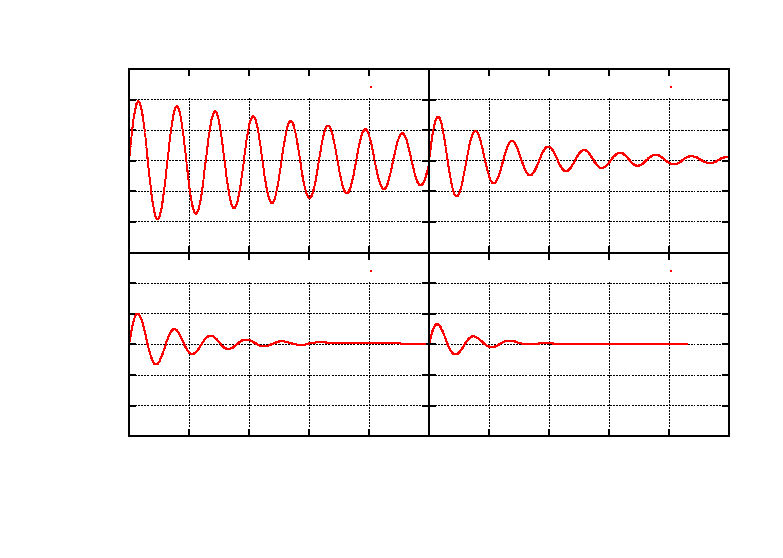
\includegraphics{plot_dif0}}%
    \gplfronttext
  \end{picture}%
\endgroup

   \caption{\small{Schwingungsverlauf des Pohlschen Rades ohne Anregung für vier verschiedene Dämpfungen}}
   \label{img:1}
\end{figure}
\ \\
Mit der Gleichung
\begin{align}
\Lambda := \rm {ln}\left[{\frac{\varphi(t)}{\varphi(t+T)}}\right]=\beta T \nonumber
\end{align}
kann das Logarithmische Dekrement berechnet werden. Dazu werden mit einem Peakfinding-Algorithmus die Maxima der Schwingung bestimmt und jeweils für zwei benachbarte Maxima das Logarithmische Dekrement berechnet. Anschließend werden die Werte gemittelt. Die Dämpfung $\beta$ ergibt sich dann durch Multiplikation mit der Periodendauer. Die Ergebnisse befinden sich ebenfalls in Tabelle \ref{tab:1}.\\
Damit lässt sich nun die ungedämpfte Eigenfrequenz über die Beziehung
\begin{align}
\omega_e = \sqrt{\omega_0^{2}-\beta^{2}}  \Leftrightarrow \omega_0 = \sqrt{\omega_e^{2}+\beta^{2}}
\end{align}
finden. Der Mittelwert über die vier Messungen ist
\begin{align}
\omega_0 = \SI{2,08\pm0,18}{\per\second} \nonumber
\end{align}
Dieser stimmt nicht überein mit der Eigenfrequenz für die Stellung "`0 mm"' der Wirbelstrombremse. Dies ist aber nicht verwunderlich, wenn man bedenkt, dass das betrachtete System selbst bei abgeschalteter Wirbelstrombremse nicht völlig reibungs- bzw. dämpfungsfrei ist. Es treten sowohl Luftreibung, als auch mechanische Reibung in den Lagern auf, was sich auch im Wert der Dämpfungskonstante niederschlägt.
\begin{table}[!htbp]
\centering
\begin{tabular}{|l|l|l|l|l|}
\hline 
Dämpfung & $\SI{0}{mm}$ & $\SI{4}{mm}$ & $\SI{6}{mm}$ & $\SI{8}{mm}$ \\
\hline
$\omega_e$ $[\SI{}{\per\second}]$ & $\SI{2,06\pm0,10}{\per\second}$ & $\SI{2,06\pm0,10}{\per\second}$ & $\SI{2,16\pm0,13}{\per\second}$ & $\SI{1,96\pm0,15}{\per\second}$ \\
\hline
$\Lambda$ & $\SI{0,112\pm0,005}{}$ & $\SI{0,38\pm0,06}{}$ & $\SI{0,80\pm0,06}{}$ & $\SI{1,5\pm0,4}{}$ \\
\hline
$\beta$ $[\SI{}{\per\second}]$ & \SI{0,037\pm0,005}{} & \SI{0,12\pm0,06}{} & \SI{0,27\pm0,06}{} & \SI{0,5\pm0,4}{} \\
%\hline
%Errechnete & & & & \\ ungedämpfte & & & & \\  Eigenfrequenz & & & & \\$\omega_0$: & ... & ... & ... & \\
\hline 
\end{tabular} 
\caption{\small{Auswertung der Schwingungen für die vier Dämpfungen ohne Anregung}}
\label{tab:1}
\end{table}
\newpage
\subsection{Schwingungen mit Anregungen}
Zunächst soll für jede Dämpfung die Resonanzkurve aufgetragen werden. Dazu  muss für jede Kombination aus Dämpfung und Erregerfrequenz die Schwingungsamplitude bestimmt werden. Dies geschieht durch Suchen der Minima/Maxima mit dem bereits erwähnten Peakfinding-Algorithmus und anschließende Mittelwertbildung. Abbildung \ref{img:2} zeigt die resultierenden Kurven für alle Dämpfungen:
\ \\
\begin{figure}[!htbp]
\centering
\input{./frequenzgang}
\caption{Das unterschiedliche Resonanzverhalten des Rades für die drei Dämpfungen in Abhängigkeit von Eigenfrequenz
und Anregungsfrequenz} 
\label{img:2}
\end{figure}
\newpage \ \\
Durch die externe Anregung des Resonators entsteht eine Phasenverschiebung $\phi$, die von der Dämpfung und der Erregerfrequenz abhängt:
\begin{align}
\phi=arctan\left(\frac{2\beta\omega}{\omega_0^{2}-\omega^{2}}\right) \nonumber
\end{align}
Trägt man die Phasenverschiebung (im Bereich zwischen 0° und 180°) gegen das Verhältnis von der Erregerfrequenz zur Eigenfrequenz des Systems auf, erhält man folgende Darstellung:
\begin{figure}[!htbp]
\input{./phasenverschiebung}
\caption{Die unterschiedlichen Phasenverschiebungen des Rades abhängig vom Verhältnis von Eigenfrequenz zu 
Anregungsfrequenz}{Anmerkung: Durch die Annäherung mit Splines entspricht der Kurvenverlauf teilweise nicht der Theorie} 
\end{figure}
\newpage \ \\
Aus Abb. \ref{img:2} lassen sich die gemessenen Resonanzfrequenzen bestimmen. Die theoretisch erwarteten Resonanzfrequenzen lassen sich aus den gemessenen Dämpfungskonstanten und Eigenfrequenzen über die Formel
\begin{align}
\omega_r = \sqrt{\omega_0^{2} - 2\beta^{2}} \nonumber
\end{align}
berechnen. Der Vergleich in Tab. \ref{tab:2} zeigt, dass die Werte im Rahmen der Fehlergenauigkeit übereinstimmen. Dies liegt zum Teil auch an den relativ großen Fehlern der berechneten Werte, welche aus der Bestimmung des Logarithmischen Dekrements resultieren. Auffällig ist, dass die erwarteten Werte mit zunehmender Dämpfung tendenziell abfallen, während die gemessenen Werte tendenziell größer werden. 
\begin{table}[!htbp]
\centering
\begin{tabular}{|c|c|c|}
\hline 
Stellung der Wirbelstrombremse & $\omega_r$ erwartet & $\omega_r$ gemessen \\ 
\hline 
$\SI{4}{mm}$ & $\SI{2.1\pm0.4}{\per\second}$ & $\SI{1.95\pm0.10}{\per\second}$ \\ 
\hline 
$\SI{6}{mm}$ & $\SI{2.1\pm0.4}{\per\second}$ & $\SI{1.98\pm0.13}{\per\second}$ \\ 
\hline 
$\SI{8}{mm}$ & $\SI{1.8\pm0.7}{\per\second}$ & $\SI{2.04\pm0.15}{\per\second}$ \\ 
\hline 
\end{tabular} 
\caption{\small{Vergleich der erwarteten und der gemessenen Resonanzfrequenzen}}
\label{tab:2}
\end{table}
\newpage
\newpage
\section{Fehlerrechnung}
\subsection{Aufnahme der Werte}
Da die Güte der verwendeten Messgeräte nicht bekannt ist, muss der Messfehler geschätzt werden. Der Auslenkungswinkel des Pohlschen Rades wird mit einer Auflösung von $\SI{0,25}{\degree}$ aufgezeichnet, daher wird ein Fehler von $\sigma_\varphi=\SI{0,125}{\degree}$ angenommen.

\subsection{Logarithmisches Dekrement}
Der Fehler bei der Berechnung des Logarithmischen Dekrements lässt sich durch eine Gaußsche Fehlerfortpflanzung ermitteln:

\begin{align}
\sigma_\Lambda=\sqrt{\sigma_{\varphi_k}^2\cdot\left( \frac{1}{\varphi_k}\right)^2+\sigma_{\varphi_{k+1}}^2\cdot\left( \frac{1}{\varphi_{k+1}}\right) ^2}
\end{align}
Da die Werte gemittelt werden, wird jeweils der größte Fehler angenommen.
\ \\
Mit einer weiteren Fehlerfortpflanzung folgt der Fehler der Dämpfungskonstante $\beta$

\begin{align}
\sigma_\beta=\sqrt{\sigma_\Lambda^2}
\end{align}

\subsection{Eigenfrequenz}
Der Fehlerfortpflanzung der ungedämpften Eigenfrequenz lautet
\begin{align}
\sigma_{\omega_0} = \sqrt{\sigma_{\omega_e}^{2}\left(\frac{\omega_e}{\sqrt{\omega_e^{2}+\beta^{2}}}\right)^{2}+\sigma_\beta^{2}\left(\frac{\beta}{\sqrt{\omega_e^{2}+\beta^{2}}}\right)^{2}}
\end{align}

\subsection{Resonanzfrequenz}
Die Gaußsche Fehlerfortpflanzung ergibt für die Resonanzfrequenz einen Fehler von
\begin{align}
\sigma_{\omega_r}=\sqrt{\sigma_{\omega_0}\frac{\omega_e}{\sqrt{\omega_e^{2}-2\beta^{2}}}+\sigma_\beta\frac{2\beta}{\sqrt{\omega_e^{2}-2\beta^{2}}}}
\end{align}

\subsection{Diskrete Fouriertransformation}
Die DFT besitzt nur eine begrenzte Auflösung, die von der Anzahl der Messwerte $N$ und der Abtastzeit $t_a$ abhängt. Die Auflösung x berechnet sich zu
\begin{align}
x = \frac{1}{N t_a}
\end{align}
Zu den Frequenzen der DFT addiert sich somit ein Fehler in der Größe der halben Auflösung. In diesem Versuch ist $t_a = \SI{15,625}{ms}$.
\newpage
\section{Diskussion}
Insgesamt war es spannend einen solchen Schwingungsprozess nochmal nachzuvollziehen und auszuwerten. Etwas erfolgreichere
Messergebnisse hätten allerdings die Motivation noch gesteigert.

\subsection{Fehlerdiskussion}
Da eventuelle Ungenauigkeiten bei der Aufnahme der Daten nicht angegeben waren, haben wir uns an der Auflösung 
der aufgezeichneten Daten orientiert, hierbei sind wir von einer \glqq fehlerfreien \grqq{} Zeitbestimmung 
ausgegangen. 
Der wesentlichste vermeidbare Fehler war gegebenenfalls zu kurzes Warten bei der Einschwingzeit, was
die Messergebnisse verfälscht haben kann. \\
Deutlich hat sicherlich der Zustand der Versuchsapparatur zu Fehlern beigetragen, was insbesondere an signifikant 
unterschiedlichen Messergebnissen an den drei Apparaturen zu sehen ist.
Auch die Tatsache dass auch bei kleinster Dämpfung die Amplitude der erzwungenen Schwingung nicht in die Nähe einer 
Resonanzkatastrophe kam spricht für Ungenauigkeiten durch Verschleiß der Apparaturen. \\
Bei der Auswertung der Messwerte hätte man die Fehler beim Logarithmischen Dekrement (sowie den davon abhängigen Werten) minimieren können, indem man weniger Maxima einbezogen (der Fehler nimmt mit kleinerer Amplitude zu) oder ein gewichtetes Mittel verwendet hätte. \\
Eine weitere Auffälligkeit ist die Verschiebung der Resonanzkurven (vgl. Abb. \ref{img:2}). Vor allem die Kurve der starken Dämpfung ist deutlich nach rechts verschoben. Die Ursache dafür könnte entweder im Verschleiß des Messaufbaus oder in der Ungenauigkeit bei der Bestimmung der Eigenfrequenz liegen. Möglicherweise ist auch die Angabe der Exzenterfrequenzen fehlerbehaftet.
\newpage
\thispagestyle{empty}
% Festlegung Art der Zitierung - Havardmethode: Abkuerzung Autor + Jahr
\bibliographystyle{plain}
\bibliography{litbank}{}
\end{document}